%!TEX root = ../../main.tex

\chapter{Icons}
\index{Icons}

Throughout the \giraf-software suite different icons will be used to reference different applications and functionalities. Refer to the sections below to see how and when to use these icons.

\section{\giraf Software Suite Icon}
\index{Icons}
The different applications in the \giraf software suite may want to refer to the software suite itself. To do this, the overall application icon seen in \figref{fig:overall_application_icon} can be used. This icon will also be used in some situations for indicating activity. \todo{Refer to a section describing activity indicators}

\begin{figure}[h]
	\centering
	
\includegraphics[scale=0.25]{placeholder}
	\caption{Overall application icon for the \giraf software suite}
	\label{fig:overall_application_icon}
\end{figure}

\section{Application-specific Icons}
\index{Icons}
Each application in the \giraf software suite must have its own icon. This icon should reflect the content and functionality of the application and must not be ambiguous. All application icons should furthermore use the icon-base seen in \figref{fig:application_specific_icon_base}. 
\\\\
Rendered icons must be available in sizes defined in the \href{http://developer.android.com/design/style/iconography.html}{Android Iconography article}. The foreground of the icon must be clear in any of these sizes. Furthermore, the icon must not appear smudged or otherwise distorted on any scale.

\begin{figure}[h]
	\centering
	
\includegraphics[width=0.15\textwidth]{application_specific_icon_base}
	\caption{Base for all application specific icon}
	\label{fig:application_specific_icon_base}
\end{figure}

\section{Icons used to represent functionality}
\index{Icons}
Specific icons may be used in buttons (See \texttt{GirafButton} in \gc) to represent functionality. The foreground of these icons must be gray-scaled and be quadratic (square). The functionality that the icon represents should be reflected in the icons itself. The icons should use the icon-base seen in \figref{fig:functionality_specific_icon_base}.

\begin{note}
	Please be aware that the actual icons should not be designed/rendered using the base as described above. Instead use the \texttt{GirafButton} from the \gc library. This will allow you to only design the actual foreground and not worry about the background (base).
\end{note}

\begin{figure}[h]
	\centering
	
\includegraphics[width=0.15\textwidth]{functionality_specific_icon_base}
	\caption{Base for all functionality-specific icons}
	\label{fig:functionality_specific_icon_base}
\end{figure}

\section{Icons and when to use them}
This section will describe the different icons that must be used throughout the applications in the \giraf software suite. Please notice that icons in this section are displayed on a button-like background. Icons may be used in different contexts if necessary.

\subsection{User Management}
\index{User management icons}
\index{Icons!User management}

\begin{longtable}{m{\textwidth-2.2cm} m{1.5cm}}
	\textbf{Switch User}: Used to indicate that the current profile can be switched & \parbox[c]{1.2cm}{
	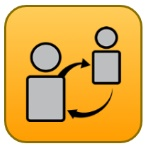
\includegraphics[width=1.2cm]{icon_examples/icon_change_user}} \\[0.6cm] \hline \\[-0.6em]

	\textbf{Back}: Used to indicate that the user can go back & \parbox[c]{1.2cm}{
	
\includegraphics[width=1.2cm]{icon_examples/icon_back}} \\[0.6cm] \hline \\[-0.6em]

	\textbf{Log out}: Used to indicate that the user can log out of the application & \parbox[c]{1.2cm}{
	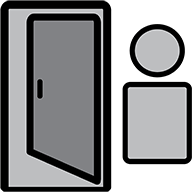
\includegraphics[width=1.2cm]{icon_examples/icon_logout}} \\[0.6cm] \hline \\[-0.6em]
\end{longtable}

\subsection{Camera}
\index{Camera icons}
\index{Icons!Camera}

\begin{longtable}{m{\textwidth-2.2cm} m{1.5cm}}
	\textbf{Camera}: Used to indicate that a camera can be used. For instance to take a picture & \parbox[c]{1.2cm}{
	
\includegraphics[width=1.2cm]{icon_examples/icon_camera}} \\[0.6cm] \hline \\[-0.6em] 

	\textbf{Switch Camera}: Used to indicate that the camera used can be switched. For instance from rear camera to front camera & \parbox[c]{1.7cm}{
	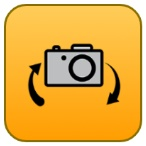
\includegraphics[width=1.2cm]{icon_examples/icon_camera_switch}} \\[0.6cm] \hline \\[-0.6em] 
\end{longtable}


\subsection{Microphone}
\index{Microphone icons}
\index{Icons!Microphone}

\begin{longtable}{m{\textwidth-2.2cm} m{1.5cm}}
	\textbf{Microphone}: Used to indicate that the microphone in the tablet may be utilized. For instance for recording speech & \parbox[c]{1.2cm}{
	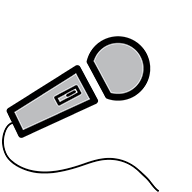
\includegraphics[width=1.2cm]{icon_examples/icon_microphone}} \\[0.6cm] \hline \\[-0.6em]

	\textbf{Microphone (off)}: Used to indicate that the microphone is unavailable & \parbox[c]{1.2cm}{
	
\includegraphics[width=1.2cm]{icon_examples/icon_microphone_off}} \\[0.6cm] \hline \\[-0.6em]

	\textbf{Microphone (on)}: Used to indicate that the microphone is currently in use & \parbox[c]{1.2cm}{
	
\includegraphics[width=1.2cm]{icon_examples/icon_microphone_on}} \\[0.6cm] \hline \\[-0.6em] 
\end{longtable}


\subsection{Media}
\index{Media icons}
\index{Icons!Media}

\begin{longtable}{m{\textwidth-2.2cm} m{1.5cm}}
	\textbf{Play}: Used to indicate that something is playing & \parbox[c]{1.2cm}{
	
\includegraphics[width=1.2cm]{icon_examples/icon_play}} \\[0.6cm] \hline \\[-0.6em]

	\textbf{Record}: Used to indicate that something is recording & \parbox[c]{1.2cm}{
	
\includegraphics[width=1.2cm]{icon_examples/icon_record}} \\[0.6cm] \hline \\[-0.6em]

	\textbf{Stop}: Used to indicate that either something playing or recording can be stopped & \parbox[c]{1.2cm}{
	
\includegraphics[width=1.2cm]{icon_examples/icon_stop}} \\[0.6cm] \hline \\[-0.6em]
\end{longtable}


\subsection{Arrows}
\index{Arrow icons}
\index{Icons!Arrows}

\todo[inline]{Consider if these should be available}

\begin{longtable}{m{\textwidth-2.2cm} m{1.5cm}}
	\textbf{Arrow (down)}: X & \parbox[c]{1.2cm}{
	
\includegraphics[width=1.2cm]{icon_examples/icon_arrow_down}} \\[0.6cm] \hline \\[-0.6em]

	\textbf{Arrow (left)}: X & \parbox[c]{1.2cm}{
	
\includegraphics[width=1.2cm]{icon_examples/icon_arrow_left}} \\[0.6cm] \hline \\[-0.6em]

	\textbf{Arrow (right)}: X & \parbox[c]{1.2cm}{
	
\includegraphics[width=1.2cm]{icon_examples/icon_arrow_right}} \\[0.6cm] \hline \\[-0.6em]

	\textbf{Arrow (up)}: X & \parbox[c]{1.2cm}{
	
\includegraphics[width=1.2cm]{icon_examples/icon_arrow_up}} \\[0.6cm] \hline \\[-0.6em]
\end{longtable}


\subsection{Version control}
\index{Version control icons}
\index{Icons!Version control}

\begin{longtable}{m{\textwidth-2.2cm} m{1.5cm}}
	\textbf{Undo}: Used to indicate that an action can be undone & \parbox[c]{1.2cm}{
	
\includegraphics[width=1.2cm]{icon_examples/icon_regret}} \\[0.6cm] \hline \\[-0.6em]

	\textbf{Redo}: Used to indicate that an undone action can be redone & \parbox[c]{1.2cm}{
	\reflectbox{
\includegraphics[width=1.2cm]{icon_examples/icon_regret}}} \\[0.6cm] \hline \\[-0.6em]

	\textbf{Synchronize}: Used to indicate that data can be synchronize to/from the server & \parbox[c]{1.2cm}{
	
\includegraphics[width=1.2cm]{icon_examples/icon_synchronize}} \\[0.6cm] \hline \\[-0.6em]

	\textbf{Save}: Used to indicate that actions performed can be saved & \parbox[c]{1.2cm}{
	
\includegraphics[width=1.2cm]{icon_examples/icon_save}} \\[0.6cm] \hline \\[-0.6em] 

	\textbf{Cancel}: Used to indicate that some action can be canceled & \parbox[c]{1.2cm}{
	
\includegraphics[width=1.2cm]{icon_examples/icon_cancel}} \\[0.6cm] \hline \\[-0.6em]
\end{longtable}


\subsection{Data Management}
\index{Data management icons}
\index{Icons!Data management}

\begin{longtable}{m{\textwidth-2.2cm} m{1.5cm}}
	\textbf{Add}: Used to indicate that a new instance of something can be created & \parbox[c]{1.2cm}{
	
\includegraphics[width=1.2cm]{icon_examples/icon_add}} \\[0.6cm] \hline \\[-0.6em]

	\textbf{Rotate}: Used to indicate that something can be rotated & \parbox[c]{1.2cm}{
	
\includegraphics[width=1.2cm]{icon_examples/icon_rotate}} \\[0.6cm] \hline \\[-0.6em]

	\textbf{Resize}: Used to indicate that something can be resized & \parbox[c]{1.2cm}{
	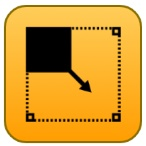
\includegraphics[width=1.2cm]{icon_examples/icon_resize}} \\[0.6cm] \hline \\[-0.6em]

	\textbf{Copy}: Used to indicate that something can be copied & \parbox[c]{1.2cm}{
	
\includegraphics[width=1.2cm]{icon_examples/icon_copy}} \\[0.6cm] \hline \\[-0.6em]

	\textbf{Edit}: Used to indicate that something can be edited & \parbox[c]{1.2cm}{
	
\includegraphics[width=1.2cm]{icon_examples/icon_edit}} \\[0.6cm] \hline \\[-0.6em]

	\textbf{Delete}: Used to indicate that something can be deleted & \parbox[c]{1.2cm}{
	
\includegraphics[width=1.2cm]{icon_examples/icon_delete}} \\[0.6cm] \hline \\[-0.6em]

	\textbf{Change Pictogram}: Used to indicate that a pictogram can be changed or set & \parbox[c]{1.2cm}{
	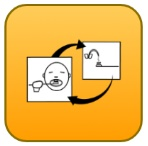
\includegraphics[width=1.2cm]{icon_examples/icon_change_picto}} \\[0.6cm] \hline \\[-0.6em]

	\textbf{Search}: Used to indicate that a search-action can be performed & \parbox[c]{1.2cm}{
	
\includegraphics[width=1.2cm]{icon_examples/icon_search}} \\[0.6cm] \hline \\[-0.6em]
\end{longtable}


\subsection{Utilities}
\index{Utility icons}
\index{Icons!Utility}

\begin{longtable}{m{\textwidth-2.2cm} m{1.5cm}}
	\textbf{Help}: Used to indicate that the user might seek help & \parbox[c]{1.2cm}{
	
\includegraphics[width=1.2cm]{icon_examples/icon_help}} \\[0.6cm] \hline \\[-0.6em]

	\textbf{Settings}: Used to indicate that the user might adjust settings & \parbox[c]{1.2cm}{
	
\includegraphics[width=1.2cm]{icon_examples/icon_settings}} \\[0.6cm] \hline \\[-0.6em]

	\textbf{Landscape to Portrait}: Used to indicate that the orientation of the tablet can be changed from landscape mode to portrait mode & \parbox[c]{1.2cm}{
	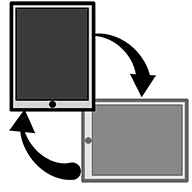
\includegraphics[width=1.2cm]{icon_examples/icon_change_land_to_port}} \\[0.6cm] \hline \\[-0.6em] 

	\textbf{Portrait to Landscape}: Used to indicate that the orientation of the tablet can be changed from portrait mode to landscape mode & \parbox[c]{1.2cm}{
	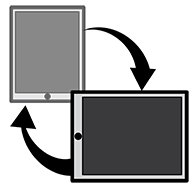
\includegraphics[width=1.2cm]{icon_examples/icon_change_port_to_land}} \\[0.6cm] \hline \\[-0.6em]

	\textbf{Give Tablet}: Used to indicate that the tablet will be given to another user & \parbox[c]{1.2cm}{
	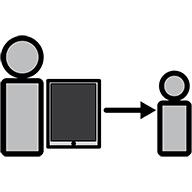
\includegraphics[width=1.2cm]{icon_examples/icon_give_tablet}} \\[0.6cm] \hline \\[-0.6em]
\end{longtable}


\subsection{Miscellaneous}
\index{Miscellaneous icons}
\index{Icons!Miscellaneous}

\begin{longtable}{m{\textwidth-2.2cm} m{1.5cm}}
	\textbf{Accept}: Used to indicate that something is accepted. For instance when user is presented with a confirmation & \parbox[c]{1.2cm}{
	
\includegraphics[width=1.2cm]{icon_examples/icon_accept}} \\[0.6cm] \hline \\[-0.6em]

	\textbf{Choose}: Used to indicate that the user should make a choice & \parbox[c]{1.2cm}{
	
\includegraphics[width=1.2cm]{icon_examples/icon_choose}} \\[0.6cm] \hline \\[-0.6em]

	\textbf{Color Background}: Used to indicate that colors of the background of an element can be specified & \parbox[c]{1.2cm}{
	
\includegraphics[width=1.2cm]{icon_examples/icon_color_background}} \\[0.6cm] \hline \\[-0.6em]

	\textbf{Color Stroke}: Used to indicate that colors of the stroke of an element can be specified & \parbox[c]{1.2cm}{
	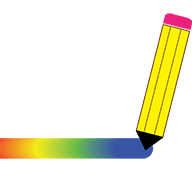
\includegraphics[width=1.2cm]{icon_examples/icon_color_stroke}} \\[0.6cm] \hline \\[-0.6em]

	\textbf{Eraser}: Used to indicate content can be erased & \parbox[c]{1.2cm}{
	
\includegraphics[width=1.2cm]{icon_examples/icon_eraser}} \\[0.6cm] \hline \\[-0.6em]
\end{longtable}